
%(BEGIN_QUESTION)
% Copyright 2006, Tony R. Kuphaldt, released under the Creative Commons Attribution License (v 1.0)
% This means you may do almost anything with this work of mine, so long as you give me proper credit

A {\it strain gauge} is a device used to measure the strain (compression or expansion) of a solid object by producing a resistance change proportional to the amount of strain.  As the gauge is strained, its electrical resistance alters slightly:

$$\includegraphics[width=15.5cm]{i00181x02.eps}$$

Explain {\it why} the electrical resistance of a strain gauge changes as it stretches and shrinks, and also correlate the direction of resistance change (more or less) with the direction of applied force.

\vskip 10pt

The following strain gauge is shown connected in a ``quarter-bridge'' circuit (meaning only one-quarter of the bridge actively senses strain, while the other three-quarters of the bridge are fixed in resistance):

$$\includegraphics[width=15.5cm]{i00181x01.eps}$$

Explain what would happen to the voltage measured across this bridge circuit ($V_{AB}$) if the strain gauge were to be {\it compressed}, assuming that the bridge begins in a balanced condition with no strain on the gauge.

\vskip 20pt \vbox{\hrule \hbox{\strut \vrule{} {\bf Suggestions for Socratic discussion} \vrule} \hrule}

\begin{itemize}
\item{} A good problem-solving technique to apply when analyzing directions of change in a Wheatstone bridge circuit is to consider {\it limiting cases}.  Instead of asking ourselves what would happen in the circuit if the strain gauge resistance changed slightly, we ask ourselves what would happen if the resistance changed {\it dramatically} (i.e. full open or full short).  Explain how we could apply this problem-solving technique to this circuit.
\item{} Strain gauges are widely used in the automotive and aerospace industries to study the strain of mechanical assemblies.  Explain how a strain gauge might be used to measure the strain of something like a truck axle.
\end{itemize}

\underbar{file i00181}
%(END_QUESTION)





%(BEGIN_ANSWER)

As a strain gauge is stretched, its conductors become longer and thinner, thus increasing resistance.  As a strain gauge is compressed, its conductors become shorter and fatter, thus decreasing resistance.  The bridge circuit becomes more unbalanced as the strain gauge's resistance changes from the neutral (resting) value.

\vskip 10pt

In this circuit, voltage drop across the strain gauge decreases as it is compressed.  This causes the potential at point A to become more negative, resulting in $V_{AB}$ developing with A negative and B positive.


%(END_ANSWER)





%(BEGIN_NOTES)






\vfil \eject

\noindent
{\bf Prep Quiz:}

A {\it strain gauge}:

\begin{itemize}
\item{} Measures applied force by changing its electrical resistance accordingly
\vskip 5pt 
\item{} Measures vibration by creating an AC voltage when shaken or accelerated
\vskip 5pt 
\item{} Indicates applied force with a dial-style face like a gauge or bathroom scale
\vskip 5pt 
\item{} Stabilizes voltage in a DC ``Wheatstone bridge'' circuit for high accuracy
\vskip 5pt 
\item{} Acts as a thermometer, sensing metal fatigue caused by temperature
\vskip 5pt 
\item{} Measures electrical resistance by changing length according to how hot it is
\end{itemize}

%INDEX% Measurement, strain gauge

%(END_NOTES)


